% Nome do capítulo
\chapter{Revisão Bibliográfica}
\label{cap:2}
\vspace{-1.9cm}

Neste capítulo serão apresentados os principais conceitos e definições da literatura sobre \ac{RNA}, Deep Learning, classificação e localização de objetos.

\section{\textit{Machine Learning}}
\label{secao:2:1}
\vspace{-.6cm}

\textit{Machine Learning} ou Aprendizado de Máquina é um campo de estudo cada vez mais recorrente na área de tecnologia. Em uma definição alternativa, pode-se dizer que ``[...]Aprendizado de Máquina é uma área de Inteligência Artificial cujo objetivo é o desenvolvimento de técnicas computacionais sobre o aprendizado bem como a construção de sistemas capazes de adquirir conhecimento de forma automática.'' \cite{monard-2003}. Entre as principais aplicações de Aprendizado de máquina, pode se destacar o reconhecimento de padrões, classificação de imagens e a mineração de dados. 

\citeonline{monard-2003} definem ainda que o aprendizado de máquina pode ser supervisionado ou não-supervisionado. Quando falamos do primeiro caso, queremos dizer que o algoritmo recebe um conjunto de dados na entrada, processa esses dados e retorna uma saída. Essa saída é comparada com um valor previamente associado à entrada, comumente conhecido como rótulo. Já no aprendizado não-supervisionado, as entradas não possuem rótulo algum, cabendo ao algoritmo fazer a distinção das diversas entradas. Geralmente, nesses casos é necessária uma análise posterior à execução do algoritmo para se entender os resultados obtidos.

O aprendizado supervisionado se divide em dois grupos menores: classificação e regressão. \citeonline{santos-2012} define que quando o problema possui um conjunto discreto de saídas e o objetivo é atribuir a qual dessas saídas a entrada pertence, se trata de um problema de classificação. \citeonline{santos-2012} define ainda que quando o objetivo é prever uma saída de valor contínuo pra uma entrada, se trata de um problema de regressão.

As seções \ref{subsecao:2:1:1} e \ref{subsecao:2:1:2} irão definir melhor esses conceitos.

\subsection{Regressão}
\label{subsecao:2:1:1}

Como definido anteriormente, o problema de regressão consiste em calcular para cada entrada uma saída que possua um valor contínuo. \citeonline{dosualdo-2003} define que a regressão consiste em fazer uma relação entre os atributos $X={x_1, x_2,..., x_n}$ - onde $X$ é o conjunto de entrada e cada $x_i$ é um atributo numérico ou quantitativo - e $Y$, tal que $Y$ é um atributo ou um conjunto de atributos meta. \citeonline{apte-1997} definem essa relação por meio da Equação  \ref{eq:eq1}.

\begin{equation}
\label{eq:eq1}
	Y = f(x_1, x_2,..., x_n)
\end{equation}

A relação entre o(s) atributo(s) $X$ e o(s) atributo(s)-meta $Y$ alcançada como resultado de um algoritmo de regressão é chamado de modelo. Após a definição do modelo é importante fazer uma avaliação para dizer o quão confiável será a predição gerada pelo modelo. Existem diversas funções usadas na avaliação dos algoritmos de regressão, e uma das mais comuns é o \ac{MSE} que é definido pela Equação  \ref{eq:eq2}.

\begin{equation}
\label{eq:eq2}
	E = \dfrac{1}{N}\sum_{i = 0}^{N}(Y_i - f(X)_i)^2
\end{equation}

\noindent
Em que $E$ é o erro, $N$ é o tamanho do conjunto de amostras, $Y_i$ é o valor esperado do atributo-meta e $f(X_i)$ é o resultado do modelo para a entrada $X_i$. O objetivo do treinamento da predição, é minimizar esse erro quadrático, de forma que - em tese - o resultado previsto seja próximo do esperado.

Alguns exemplos de problemas de regressão são: 

\begin{enumerate}
	\item Predizer o percentual de gordura que uma pessoa possui no corpo, recebendo como entrada atributos como altura, idade, peso, sexo \cite{dosualdo-2003};
	\item Predizer o preço de um imóvel baseado em atributos como o tamanho, número de cômodos, número de quartos, etc. \cite{pereira-2012}.
\end{enumerate}

Uma grande limitação nos métodos de regressão é que eles em sua maioria solucionam problemas que possuem apenas um atributo-meta. Porém, os métodos de regressão baseados em \ac{RNA} podem retornar múltiplos resultados. Esse termo será definido na Sessão \ref{secao:2:2}.

\subsection{Classificação}
\label{subsecao:2:1:2}

Como mencionado anteriormente, o problema de classificação consiste em fazer uma predição quando as saídas são discretas. A ideia dos algoritmos de classificação é definir para cada entrada, um rótulo ou classe no meio de um conjunto finito de rótulos. Um método estatístico muito utilizado nos problemas de classificação é a regressão logística. A regressão logística é bem similar à regressão linear, com a diferença que o resultado é um número entre zero e um, configurando na verdade, a probabilidade de, dado uma entrada $X$ tal que $X = {x_1, x_2, ..., x_n}$ gerar uma saída verdadeira para a hipótese $Y$. Normalmente, os modelos de regressão logística aplicam a função sigmóide, descrita pela Equação  \ref{eq:eq3}.

\begin{equation}
\label{eq:eq3}
Y = \dfrac{1}{1 + e^{-g(X)}}
\end{equation}

A regressão logística se ajusta muito bem a problemas de classificação binária. Porém, a grande maioria dos problemas de classificação possuem mais de uma classe, consistindo então em dizer para uma entrada $X$ tal que $X = [x_1, x_2, ..., x_n]$ a qual classe de $Y$ ela pertence, tal que $Y = [y_1, y_2, ..., y_m]$. \citeonline{Thanh-2015} afirmam que as principais abordagens para solucionar problemas de classificação com $M$ classes consistem em dividir o problema em vários problemas de classificação binária.

Essa divisão pode ser feita de duas formas diferentes: 
\begin{itemize}
	\item A primeira consiste em gerar $M - 1$ problemas de classificação binária e resolver cada um de forma independente. Após resolver os problemas de classificação, determinar a classe final a partir das probabilidades obtidas selecionando a classe que obteve a maior probabilidade. Essa abordagem é conhecida como \textit{one-versus-all}.
	\item A segunda consiste em combinar as classes em pares e, para cada par de classe gerar um problema de classificação. Isto é, seja $Y$ um conjunto de classes, para cada classe $y \in Y$ criar um problema de classificação para $y$ e  cada $y_\beta$ tal que $y_\beta \in Y - [y]$. Isso gera um conjunto de $\frac{M (M - 1)}{2}$ problemas de classificação. Após gerar e solucionar os problemas, o resultado será a classe que for mais vezes selecionada.
\end{itemize}

Com base na primeira abordagem, começou a ser utilizada uma função para os problemas de classificação que envolvem múltiplas classes. Essa função é a \textit{softmax} que calcula o valor de cada saída e divide pela soma das saídas, gerando assim uma saída normalizada que corresponde à probabilidade de o dado de entrada estar na classe. Atualmente é a função mais utilizada para problemas de classificação com múltiplas classes e é descrita pela Equação  \ref{eq:eq4}.

\begin{equation}
\label{eq:eq4}
	f(x)_i = \dfrac{e^{\beta x_i}}{\sum_{j = 1}^{K}e^{\beta x_j}} \forall i = 1,...,K e x = {x_1, ... ,x_k} \in X^K
\end{equation}

Assim como na regressão linear, a perda na regressão logística pode ser calculado pelo \ac{MSE}. Porém, com o tempo, surgiram outras funções que calculam a perda de forma mais eficiente em problemas de classificação.

\section{Redes Neurais Artificiais}
\label{secao:2:2}

As \ac{RNA}s são uma das principais técnicas de aprendizagem de máquina e podem ser implementadas tanto para problemas supervisionados, quanto não-supervisionados. \citeonline{jost-2015} definiu as \ac{RNA}s da seguinte forma:

\begin{citacao}
	As \ac{RNA}s possuem inspiração nas redes neurais biológicas, constituídas de neurônios separados por camadas, que processam informações e estão conectados via pesos sinápticos, sendo na maioria das vezes sistemas adaptativos que modificam sua estrutura através de informações, que fluem pela rede durante a etapa de aprendizado \cite{jost-2015}.
\end{citacao}

Além disso, é importante mencionar que em uma rede neural, existem duas camadas em particular que são muito importantes: a primeira camada, que é a camada de entrada de dados, e a última camada que é a camada de saída. Existem dois tipos de \ac{RNA}s: as redes \textit{feed forward}, que processa apenas o estado atual das entradas, e as redes neurais recorrentes que processa o estado atual e o estado anterior. As redes neurais recorrentes podem ser usadas de forma eficiente para processar vídeos, séries temporais e outros dados que possuam múltiplos estados.

A \ac{RNA} \textit{feed forward} mais básica que existe é a \textit{Perceptron}, composta apenas por um conjunto de neurônios de entrada e um único neurônio de saída. A Equação  \ref{eq:eq5} representa a fórmula de um \textit{Perceptron}, onde $n$ é o número de entradas, $W_i$ são os respectivos pesos de cada entrada, $X_i$ são as entradas e $B$ é o viés do neurônio.

\begin{equation}
Y=\Big(\sum_{i=1}^{n}{(W_i \times X_i)}\Big) - B
\label{eq:eq5}
\end{equation}

Uma rede percepron não é uma arquitetura de redes neurais artificiais muito poderosa, mas deu base para outras arquiteturas mais robustas. A principal delas é o \textit{Perceptron} Multi-Camadas.

\subsection{\textit{Multi-Layer Perceptron}}
\label{subsecao:2:2:1}


As redes \textit{Perceptron} Multicamadas ou \ac{MLP} são baseadas nos \textit{Perceptron}s simples, como mencionado anteriormente. A diferença, porém, é que elas trabalham com mais camadas do que simplesmente as camadas de entrada e saída. Geralmente elas possuem uma ou duas camadas intermediárias às camadas externas. Essas camadas intermediárias, também são chamadas de camadas ocultas e servem para conferir uma robustez maior ao método.

Nas \ac{MLP}s, uma outra diferença é que as funções de ativação podem variar. As mais comuns são o \ac{ReLU} (definido pela Equação  \ref{eq:eq6}), a função sigmóide (descrita na Seção \ref{subsecao:2:1:2}) e a tangente hiperbólica (definida pela Equação  \ref{eq:eq7}).

\begin{equation}
	Y(x) = max(0, x)
	\label{eq:eq6}
\end{equation}

\begin{equation}
	Y(x) = \dfrac{e^x - e^{-x}}{e^x+e^{-x}}
	\label{eq:eq7}
\end{equation}

Como foi dito anteriormente, a \ac{MLP} trabalha com aprendizado supervisionado, isso quer dizer que os dados que ela opera são rotulados, e tem uma saída esperada. Quando as entradas são processadas e os resultados das saídas são calculados, eles são comparados com os valores esperados pelos rótulos e é gerado a função de erro quadrático, definida na Seção \ref{subsecao:2:1:1}.

Sabendo-se disso, o objetivo para melhorar a precisão da \ac{MLP} é minimizar o valor da função erro, ou seja, tornar as saídas da rede o mais próximo possível das saídas esperadas. Para tanto, é utilizado o método de retropropagação de erro que reajusta os pesos da rede de acordo com os valores obtidos usando a descida de gradiente.

\citeonline{arnold-2011} definem que aumentar o número de camadas em um \ac{MLP} não garante uma melhoria dos resultados, pois a descida de gradiente pode chegar a um mínimo local. Além disso, o aumento do número de camadas implica em um tempo muito maior de processamento. Para lidar com esse problema surge o \emph{Deep Learning}, uma arquitetura avançada com múltiplas camadas, que soluciona a dificuldade que as redes neurais possuem ao lidar com dados de alta dimensionalidade \cite{arnold-2011}.

\section{\textit{Deep Learning}}
\label{secao:2:3}

A principio não parecia ser viável manipular arquiteturas profundas de redes neurais. Porém, de acordo com \citeonline{deng-2014}, surgiu um algoritmo de aprendizado não-supervisionado que conseguiu aliviar empiricamente as dificuldades de otimização em arquiteturas profundas. Esse algoritmo é a \ac{DBN}, um modelo generativo profundo composto de uma camada visível e várias camadas ocultas compostas por uma pilha de \ac{RBM}s.

\citeonline{deng-2014} definem ainda que o aprendizado nas \ac{DBN}s é feito por um algoritmo guloso que ajusta os pesos camada-por-camada com uma complexidade linear ao tamanho e à profundidade da rede. E uma relação inesperada entre as \ac{DBN}s e as \ac{MLP}s surgiu quando descobriu-se que ao utilizar os pesos de uma \ac{DBN} com arquitetura correspondente, você consegue inicializar os pesos de uma \ac{MLP} de forma a produzir melhores resultados do que utilizando pesos aleatórios.

Uma segunda alternativa para trabalhar com aumento de camadas é o empilhamento de auto-codificadores. O empilhamento de auto-codificadores consiste basicamente em inserir na saída de uma rede neural uma segunda rede neural que para cada entrada produz uma saída específica e retreinar a nova rede neural utilizando o algoritmo de retropropagação de erro \cite{deng-2014}.

\subsection{Redes Neurais Convolucionais}
\label{subsecao:2:3:1}

As \ac{CNN} são um modelo específico de \textit{Deep Learning} muito utilizados em aplicações de visão computacional e aplicações de reconhecimento de imagens. De acordo com \citeonline{ferreira-2017}, as \ac{CNN}s utilizam matrizes para processar as entradas de dados, sendo essas matrizes unidimensionais para sinais e sequências, bidimensionais para imagens e tridimensionais para imagens volumétricas e vídeos. 

Ao contrário das \ac{RNA}s tradicionais (como \ac{MLP}), as \ac{CNN}s não necessariamente ligam todos os neurônios na camada de origem a todos os neurônios da camada de destino. \citeonline{ferreira-2017} define que existem três tipos comuns de camadas utilizadas nas redes neurais convolucionais: as camadas de convolução, camadas de \textit{pooling} e camadas completamente conexas.

A ideia da camada de convolução é de que cada neurônio recebe como entrada neurônios próximos e tem por objetivo criar mapas e filtros. \citeonline{ferreira-2017} define que em aplicações de reconhecimento de objetos, por exemplo, é comum as primeiras camadas de convolução detectarem bordas ou manchas que seriam as características mais básicas da imagem. As camadas de convolução mais profundas detectam outras características mais específicas.

Uma camada de convolução possui alguns atributos essenciais. O primeiro deles, é o tamanho do filtro. Nas principais \ac{CNN}s os filtros geralmente são $1 \times 1$ ou $3 \times 3$, porém algumas redes podem possuir filtros maiores como $5 \times 5$ ou $7 \times 7$. O segundo parâmetro é o \textit{stride} que define o tamanho do salto que será feito pelo filtro durante as operações de convolução. No processamento digital de imagens normalmente esse salto é de um \textit{pixel}, porém, nas \ac{CNN}s pode ser vantajoso dar saltos maiores. 

O último parâmetro é o \textit{padding}. O \textit{padding} consistem em preencher os cantos da imagem com zeros, de forma a aumentar o tamanho da imagem sem alterar o seu conteúdo. Esse preenchimento pode ser feito por duas razões principais: a primeira delas é porque as operações de convolução reduzem o tamanho da imagem e a principal forma de evitar essa redução de tamanho é o uso de \textit{padding}; a segunda razão também tem a ver com a redução de tamanho. Algumas vezes, é necessário reduzir o tamanho dos mapas em uma rede convolutiva, e neste sentido, as camadas de convolução (ou de \textit{pooling}) atuam fazendo o \textit{downsample} - ou redução de amostragem. Mas, em alguns casos o tamanho da saída não será um valor inteiro, sendo necessária uma correção. Essa correção pode ser feita via corte - quando uma ou mais linhas ou colunas são cortadas durante a convolução - ou por preenchimento, quando uma ou mais linhas ou colunas de zeros são acrescentadas. O corte e o preenchimento são chamados respectivamente de \textit{padding} válido e \textit{padding} equivalente. 

Sempre ligada a uma camada de convolução, é comum ter uma camada com função de ativação. Essas camadas geralmente usam as mesmas funções descritas na Seção \ref{subsecao:2:2:1}.

As camadas de \textit{pooling} são utilizadas para reduzir a dimensão de dados vindo das camadas de convolução, consequentemente reduzindo o custo computacional \cite{ferreira-2017}. Na prática elas funcionam como as camadas de convolução, mas ao invés de fazer a operação tradicional de convolução, elas reduzem um conjunto de elementos a um único representante com base em uma função específica. As funções mais utilizadas são máximo e média \cite{ferreira-2017}.

Por fim, as camadas completamente conexas são exatamente iguais às redes MLP e é comum utilizá-las no final da rede para conectar à saída. Seu acréscimo no final é importante pois faz a ligação de todos os filtros \cite{ferreira-2017}. As arquiteturas de \ac{CNN}s geralmente intercalam algumas camadas de convolução com uma camada de \textit{pooling}. As arquiteturas mais antigas costumavam adicionar camadas completamente conexas ao final, porém, os modelos mais novos, como a \ac{ResNet} e a \ac{DenseNet} já não usam mais esse conceito.

As Redes Neurais Covolucionais têm se tornado cada vez mais populares em tarefas relacionadas a processamento digital de imagens devido aos resultados que têm alcançado. A primeira \ac{CNN} usada para a tarefa de classificação de imagens foi a AlexNet proposta por \citeonline{krizhevsky-2012}. Essa rede venceu o \ac{ILSVRC} de 2012. Desde então, várias arquiteturas vêm alcançando resultados cada vez mais expressivos nessa área, como a VGG \cite{simonyan-2014}, Inception \cite{szegedy-2015}, \ac{ResNet} \cite{he-2016}, \ac{DenseNet} \cite{liu-2017}, etc..

Uma outra área impactada pelo uso das \ac{CNN}s é a área de segmentação semântica. \citeonline{long-2014} propuseram o uso de uma \ac{FCN} para fazer segmentação semântica e conseguiram obter resultados superiores ao estado da arte, utilizando camadas de deconvolução para aumentar a resolução dos mapas de filtros gerados na saída da \ac{CNN}. \citeonline{noh:2015} propuseram um trabalho mais avançado de forma a tratar algumas limitações encontradas por \citeonline{long-2014}. Essa arquitetura funciona com a estrutura de um \textit{autoencoder}, usando as camadas de deconvolução que não servem para aumentar a resolução, mas para recuperar as informações da imagem de forma mais refinada, de forma a melhorar os resultados da segmentação.

%%% p2 Escrever sobre os resultados obtidos pelas CNNs em Localização de Objetos
Nas tarefas de localização de objetos as \ac{CNN}s também têm se destacado com bons resultados. \citeonline{redmon-2015} propuseram o \ac{YOLO} e obtiveram um bom resultado fazendo localização e classificação de objetos em tempo real, conseguindo processar 45 \ac{FPS} com uma \ac{mAP} de 63,4\%. \citeonline{sren-2017} propuseram o \ac{R-CNN} e conseguiram obter resultados significativamente melhores para as tarefas de localização e classificação chegando a uma \ac{mAP} de até 78,8\%. Numa implementação alternativa com o enfoque no processamento em tempo real, a \ac{mAP} cai um pouco, chegando a 73,2\% porém, ele processa apenas 7 \ac{FPS}. Outros trabalhos que se destacam em localização e classificação de objetos é o \ac{SSD} e o \ac{DSSD}. As Seções \ref{secao:3:2} e \ref{secao:3:3} falam mais sobre eles.

\subsection{Regularização}
\label{subsecao:2:3:2}

\citeonline{caelles-2017} definem que um grande problema de trabalhar com modelos de \textit{Deep Learning} é a necessidade de um grande volume de dados para que o modelo possa generalizar bem. Do contrário, pode acontecer \textit{Overfitting}. Em \textit{Deep Learning}, \textit{Overfitting} é quando o modelo aprende a resolver o problema apenas no conjunto de dados de treinamento, isto é, gera uma solução pouco genérica.

\citeonline{goodfellow-2016} definem que uma das principais formas de evitar o \textit{Overfitting} são as técnicas de regularização. Essas técnicas criam certas restrições dentro do modelo, e essas restrições dificultam a ocorrência do \textit{Overfitting}.

\citeonline{ioffe-2015} propuseram uma técnica de regularização que se ajustou muito bem em redes neurais convolutivas e melhoraram os resultados da \textit{Inception} \cite{szegedy-2015} no desafio da \ac{ILSVRC}. Essa Técnica foi o \textit{Batch Normalization}, e ela consiste, basicamente em subtrair a média do lote de processamento da função de ativação, e dividir o resultado pelo desvio padrão. Desde que proposto, o \textit{Batch Normalization} se tornou presente nas arquiteturas mais profundas que surgiram depois, como \ac{ResNet} \cite{he-2016} e \ac{DenseNet} \cite{liu-2017}.

\citeonline{shorten-2019} definem que uma outra forma de resolver o problema do \textit{Overfitting} é tratar o problema em sua raíz: o conjunto de dados. Uma das principais causas do \textit{Overfitting} é uma base de dados pequena ou desbalanceada. Sendo assim, a principal forma de tratar o \textit{Overfitting} na basede dados é o \textit{Data Augmentation}. Essa técnica consiste em gerar dados artificiais com base nos dados reais. Em imagens, fazer \textit{Data Augmentation} é relativamente simples, pois, você pode aplicar diversas transformações em uma mesma imagem, e o \textit{ground-truth} normalmente será o mesmo. Em algumas tarefas, como segmentação ou localização, para fazer \textit{Data Augmentation} as transformações especiais que a imagem sofre (como corte ou \textit{zoom}) precisam ser aplicadas também no  \textit{ground-truth}. A Figura \ref{fig:data-aug} mostra exemplos de \textit{Data Augmentation} quando são aplicadas transformações nas cores da imagem.


  \begin{figure}[H]
  % Alterar espaçamentos antes e depois do caption
  \setlength{\abovecaptionskip}{0pt}
  \setlength{\belowcaptionskip}{0pt}
  % Caption
  \caption[Exemplos de \textit{Data Augmentation}]{Exemplos de \textit{Data Augmentation}}
  \centering
  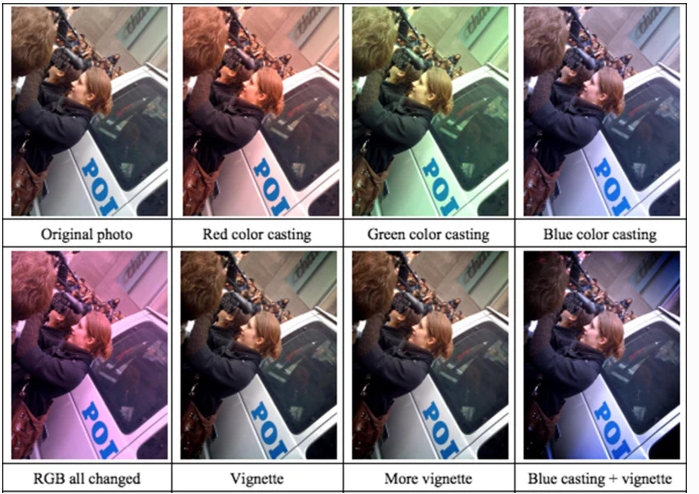
\includegraphics[width=.5\textwidth]{imagem/0x_data-augmentation.png}
% Caption centralizada
  \captionsetup{justification=centering}
  \captionfont{\small{\textbf{\\Fonte: \citeonline{shorten-2019}}}}	
  \label{fig:data-aug}
 \end{figure}

%% Citar para falar de data augmentation. https://journalofbigdata.springeropen.com/articles/10.1186/s40537-019-0197-0
%%%%%%%%%%%%%%%%%%% Formato para a inserção de figuras

%  \begin{figure}[H]
  % Alterar espaçamentos antes e depois do caption
%  \setlength{\abovecaptionskip}{0pt}
%  \setlength{\belowcaptionskip}{0pt}
  % Caption
%  \caption[Principais componentes de WiNoCs]{Principais componentes de WiNoCs}
%  \centering
%  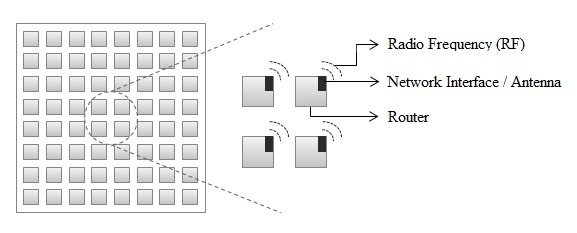
\includegraphics[width=.85\textwidth]{imagem/winoc.jpg}
  % Caption centralizada
%  \captionsetup{justification=centering}
%  \captionfont{\small{\textbf{\\Fonte: \cite{OliveiraIadis:2011}}}}	
%  \label{fig:ComponentesWiNoC}
%  \end{figure}


%%%%%%%%%%%%%%%%%%%%%%%%%% Modelo para inserir gráficos

%\begin{grafico}[H]
  % Alterar espaçamentos antes e depois do caption
%  \setlength{\abovecaptionskip}{5pt}
%  \setlength{\belowcaptionskip}{0pt}
  % Caption
%  \caption[Percentual de pacotes enviados]
%	  {Percentual de pacotes enviados}
%  \centering
%  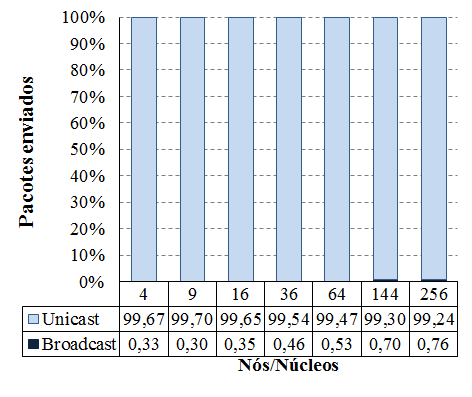
\includegraphics[width=.48\textwidth]{imagem/graficos/grafico_pacotes_enviados_bt.png}
  % Caption centralizada
%  \captionsetup[grafico]{justification=centering}
  % Fonte
%  \captionfont{\small{\textbf{\\Fonte: Dados da pesquisa}}}
%  \end{grafico}


%\begin{grafico}[H]
  % Alterar espaçamentos antes e depois do caption
%  \setlength{\abovecaptionskip}{5pt}
%  \setlength{\belowcaptionskip}{0pt}
  % Caption
%  \caption[Resultados da carga de trabalho 1]
%	  {Resultados da carga de trabalho 1}
%  \centering
%  \subfloat[Enviados]
%      {\label{graf:enviados_bt}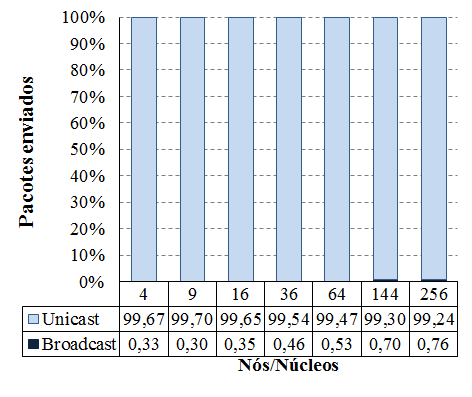
\includegraphics[width=.48\textwidth]{imagem/graficos/grafico_pacotes_enviados_bt.png}} \quad
%  \subfloat[Perdidos]
%      {\label{graf:perdidos_bt}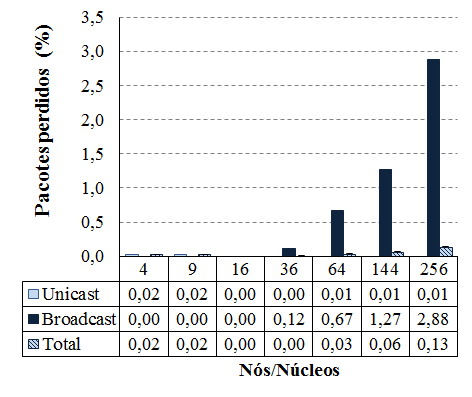
\includegraphics[width=.48\textwidth]{imagem/graficos/grafico_pacotes_perdidos_bt.png}} \quad
%  \subfloat[Taxa de injeção]
%      {\label{graf:injecao_bt}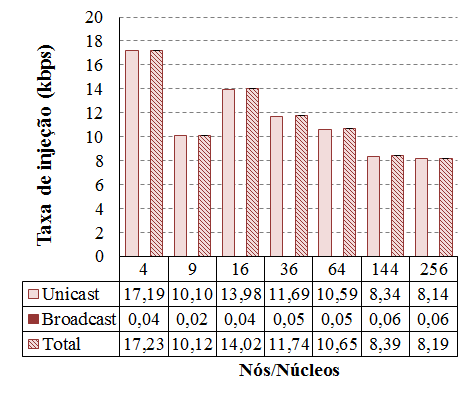
\includegraphics[width=.48\textwidth]{imagem/graficos/grafico_taxa_injecao_bt.png}} \quad
%  \subfloat[Vazão]
%      {\label{graf:vazao_bt}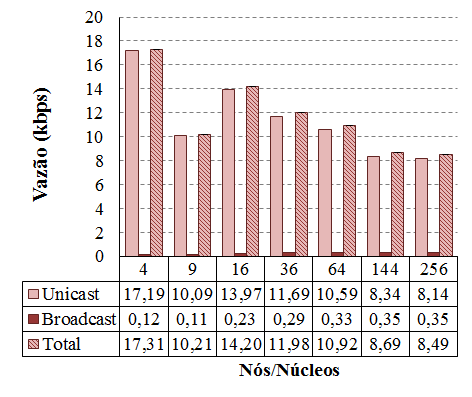
\includegraphics[width=.48\textwidth]{imagem/graficos/grafico_vazao_bt.png}}
  % Caption centralizada
%  \captionsetup[grafico]{justification=centering}
  % Fonte
%  \captionfont{\small{\textbf{\\Fonte: Dados da pesquisa}}}
%  \label{graf:quad}
%  \end{grafico}

%%%%%%%%%%%%%%%%%%%%%%%% Exemplo de criação de tabelas

   % Tabela
%  \begin{table}[H]
%    \centering
%    \footnotesize
    % Alterar espaçamentos antes e depois do caption
%    \setlength{\abovecaptionskip}{0pt}
%    \setlength{\belowcaptionskip}{0pt}
    % Caption
%    \caption[Parâmetros definidos por classe]{Parâmetros definidos por classe}
%    \label{tab:classesNas}
    % Conteúdo da tabela
%    \begin{tabular}{c|c|c|c|c|c|c|c}
%	\hline \hline
%	\textit{Benchmark} &	Parâmetro &	Classe S &	Classe W &	Classe A &	Classe B &	Classe C &	Classe D \\ 
%	\hline \hline
% 	BT & \textit{Grid}	& $12^3$	& $24^3$ 	& $64^3$	& $102^3$ 	& $162^3$	& $408^3$ \\ 
%	CG & Linhas		& 1400		& 7000 		& 14000 	& 75000 	& 150000 	& 1500000 \\ 
%	EP & Pares 		& $2^{24}$	& $2^{25}$	& $2^{28}$	& $2^{30}$	& $2^{32}$	& $2^{36}$ \\
%	FT & \textit{Grid}	& $64^3$	& $128^2*32$	& $256^2*128$	& $512*256^2$	& $512^3$	& $2048*1024^2$ \\ 
%	IS & Chaves		& $2^{16}$	& $2^{20}$	& $2^{23}$	& $2^{25}$	& $2^{27}$	& $2^{31}$ \\ 
%	LU & \textit{Grid}	& $12^3$	& $33^3$	& $64^3$	& $102^3$	& $162^3$	& $408^3$ \\
%	MG & \textit{Grid}	& $32^3$	& $128^3$	& $256^3$	& $256^3$	& $512^3$	& $1024^3$ \\ 
%	SP & \textit{Grid}	& $12^3$	& $36^3$	& $64^3$	& $102^3$	& $162^3$	& $408^3$ \\
%	\hline \hline
%    \end{tabular}
    % Fonte
%    \captionfont{\small{\textbf{\\Fonte: Adaptado de \cite{Nas:2011}}}}
%  \end{table}